%==============================================================
% 日本計算機統計学会シンポジウム 論文集用原稿テンプレート
%==============================================================

% A4用紙、本文10ptのjarticleクラスを指定
\documentclass[a4paper, 10pt]{jarticle}

% --- パッケージの読み込み ---
\usepackage[dvipdfmx]{graphicx}
\usepackage{amsmath}  % 数式環境に必要

%---【必須設定1】マージン（余白）の設定 ---
% geometryパッケージを使用
% 上下25mm以上、左右20mm以上に設定 
\usepackage[
  top=25mm,
  bottom=25mm,
  left=20mm,
  right=20mm
]{geometry}

%---【必須設定2】ページ番号を消す --- 
\pagestyle{empty}

\begin{document}

%---【必須設定3】題目、所属、氏名 ---
% 太字・中央揃えで記述 
\begin{center}
  \bfseries % これ以降を太字にする
  {\Large 状態空間モデルを用いた日本国内の宅配便取扱数における構造変化分析} % \Largeなどで文字サイズを調整

  \vspace{1.5ex} 

  中央大学大学院理工学研究科 寺嶋風雅 \\ 
\end{center}

\vspace{3ex} % 本文との間隔を空ける

%--- ここから本文 ---
\section{はじめに} 
本研究は、先行研究のSARIMAモデルでは困難であった外部イベントの定量的評価を目的とし、
状態空間モデルを日本国内の宅配便貨物の取扱量（2002-2022年）に適用した。モデルにはトレンドと季節性に加え、
2017年の運賃値上げと、複数のフェーズに分けたコロナ禍のインパクトを外生変数として組み込んだ。AICによる比較の結果、
コロナ禍を複数フェーズで捉えたモデルが最も優れていることを確認した。
本稿は、状態空間モデルが複雑なイベント効果を分離・評価する上で有効であることを実証し、
物流動向のより正確な把握に貢献するものである。

\section{分析手法} 
\subsection{使用データ} % ← ここに新しいサブセクションを追加

本研究で使用するデータは, 国土交通省が公表する「交通関係統計資料」から取得した, 2002年4月から2022年7月までの月次データである. 
先行研究（赤羽根, 2024）において構築されたデータセットを利用した. 
主要な変数を表\ref{tab:data_columns}に示す. 

\begin{table}[htbp]
  \centering
  \caption{主要変数一覧}
  \label{tab:data_columns}
  % \resizeboxでtabular環境を囲む
  \resizebox{0.5\textwidth}{!}{%
    \begin{tabular}{ll}
      \hline
      カラム名 & 内容 \\
      \hline
      \texttt{label} & 年月 (YYYY-MM-DD) \\
      \texttt{year} & 年 \\
      \texttt{month} & 月 \\
      \texttt{Transport\_tonnage} & 輸送トン数（トン） \\
      \texttt{number\_parcels} & 宅配便取扱個数（千個） \\
      \texttt{Number\_companies\_1} & 輸送トン数の調査会社数（社） \\
      \texttt{Number\_companies\_2} & 宅配便取扱個数の調査会社数（社） \\
      \hline
    \end{tabular}%
  }
\end{table}
変動を安定させるため, 本分析の目的変数には, \texttt{number\_parcels}の自然対数を取った値を用いた.
\subsection{分析モデル}
本研究で用いた状態空間モデルは, 以下のシステムモデルおよび観測モデルによって表現される. 

\begin{align}
    x_t &= F_t x_{t-1} + G_t \eta_{t} \label{eq:system_model} \\
    y_t &= H_t x_t + \beta d_t + \epsilon_t \label{eq:observation_model}
\end{align}

ここで, $x_t$は状態ベクトル, $y_t$は観測値を表す. 
状態攪乱項 $\eta_t$ および観測攪乱項 $\epsilon_t$ は, それぞれ以下の正規分布に従うと仮定する. 

\begin{equation}
    \begin{bmatrix}
      \eta_{\mu_{t}}  \\
      \eta_{\gamma_{t}}
    \end{bmatrix}
    \sim N \left( 0, 
    \begin{bmatrix}
      \sigma_{\mu_{t}}^2 & 0  \\
      0 & \sigma_{\gamma_{t}}^2
    \end{bmatrix} \right) \label{eq:eta_dist}
\end{equation}

\begin{equation}
    \epsilon_t \sim N( 0, \sigma_{\epsilon_{t}}^2) \label{eq:epsilon_dist}
\end{equation}

ここで、状態ベクトル$x_t$は、トレンド成分と周期12の季節成分から構成される。

\subsection{外生変数の設計}
本研究で用いる状態空間モデルは、トレンドや季節性といった内部構造に加え、外部からのイベントが時系列に与える影響を分離して分析できる点が特徴である。
ここでは、観測方程式に組み込む外生変数$d_t$
 の具体的な設計について述べる。

宅配便の取扱個数は、社会・経済情勢の変化に敏感に反応すると考えられる。
特に、分析対象期間中には、業界全体に影響を及ぼした大規模な運賃値上げと、
人々の生活様式を大きく変容させた新型コロナウイルス感染症（COVID-19）のパンデミックという2つの重要なイベントが発生した。
これらの影響を適切にモデル化するため、本研究ではイベントの性質に応じて期間を設定したダミー変数を設計し、外生変数として導入する。
各ダミー変数は、イベントが発生している期間は1、それ以外の期間は0をとるバイナリ変数である。
モデルは、これらの変数に対する係数$\beta$を推定することで、各イベントが宅配便取扱個数に与えた瞬間的なインパクトの大きさを定量的に評価する。
具体的な変数設計は表\ref{tab:dummy_variables}に示す通りである。
\begin{table}[htbp]
  \centering
  \caption{外生変数として導入するダミー変数一覧}
  \label{tab:dummy_variables}
  \resizebox{\textwidth}{!}{
    \begin{tabular}{llp{11cm}}
      \hline
      変数名 & 対象期間 & 説明 \\
      \hline
      \texttt{hike\_dummy} & 2017/10 -- 2019/12 & 2017年10月に実施された主要各社の運賃値上げの影響を捉えるための変数。 \\
      \texttt{covid\_main} & 2020/03 -- & COVID-19パンデミックによる巣ごもり需要の定着など、市場構造そのものに与えた持続的な変化（構造変化）を捉える変数。 \\
      \texttt{covid\_wave1} & 2020/04 -- 2020/05 & 緊急事態宣言下での急激な需要増など、パンデミック初期の短期的なインパクトを捉える変数。 \\
      \texttt{covid\_2021} & 2021/01 -- 2021/09 & 感染再拡大に伴う断続的な需要増の影響を捉える変数。 \\
      \hline
    \end{tabular}%
  }
\end{table}

\subsection{比較モデル}
本研究で採用する最終モデルの優位性、および各外部イベントが与える影響の重要性を評価するため、以下の3つの状態空間モデルを構築し、比較検討を行った。
各モデルは、2.2節で述べた基本構造を共有しつつ、2.3節で設計した外生変数の組み込み方が異なる。

\begin{itemize}
    \item \textbf{ベースラインモデル}: ローカル線形トレンド成分と季節成分のみで構成されるモデル。
    外部イベントの影響を一切考慮しない、最も基本的なモデルであり、分析の基準点となる。
    \item \textbf{単純イベントモデル}: ベースラインモデルに加え、運賃値上げダミーと、
    コロナ禍の影響を単一のダミー変数（\texttt{covid\_main}）のみで表現したモデル。イベントの影響を単純化した形で評価する。
    \item \textbf{提案モデル}: ベースラインモデルに加え、運賃値上げダミーと、
    コロナ禍の影響をその性質に応じて複数のフェーズに分けたダミー変数群（\texttt{covid\_main}, \texttt{covid\_wave1}, \texttt{covid\_2021}）
    を全て組み込んだ、本研究における提案モデルである。
\end{itemize}

これらの3モデルをそれぞれ推定し、モデルの当てはまりの良さを情報量規準AICによって評価した。
その比較結果は次章で詳述する。

\section{分析結果}
\subsection{モデルの比較と選択}
% ここに、AICの比較表などを載せ、なぜ最終モデルを選んだかを記述します。
% 例：「表Xに示す通り、提案モデルのAICが最も低かったため、これを最終モデルとして採択する。」
\begin{table}[htbp]
  \centering
  \caption{モデルの比較}
  \label{tab:model_comparison}
  \begin{tabular}{lccc}
    \hline
    モデル & 対数尤度 & AIC & BIC \\
    \hline
    1. ベースラインモデル & 471.9 & -913.9 & -861.4 \\
    2. 単純イベントモデル & 477.5 & -915.0 & -855.1 \\
    \textbf{3. 提案モデル} & \textbf{480.9} & \textbf{-919.9} & \textbf{-846.4} \\
    \hline
  \end{tabular}
\end{table}

\subsection{最終モデルの推定結果}
% ここに、最終モデルのサマリー表（各係数の推定値やp値）を載せ、
% 統計的に有意だった効果などを文章でハイライトします。

\subsection{時系列の成分分解}
% ここに、最終モデルによる分解グラフを載せ、
% トレンドや季節性、イベント効果がどのように現れているかを視覚的に説明します。
提案モデルによる分解結果を \ref{fig:Decomposition_series} に示す. 
\begin{figure}[htbp]
  \centering
  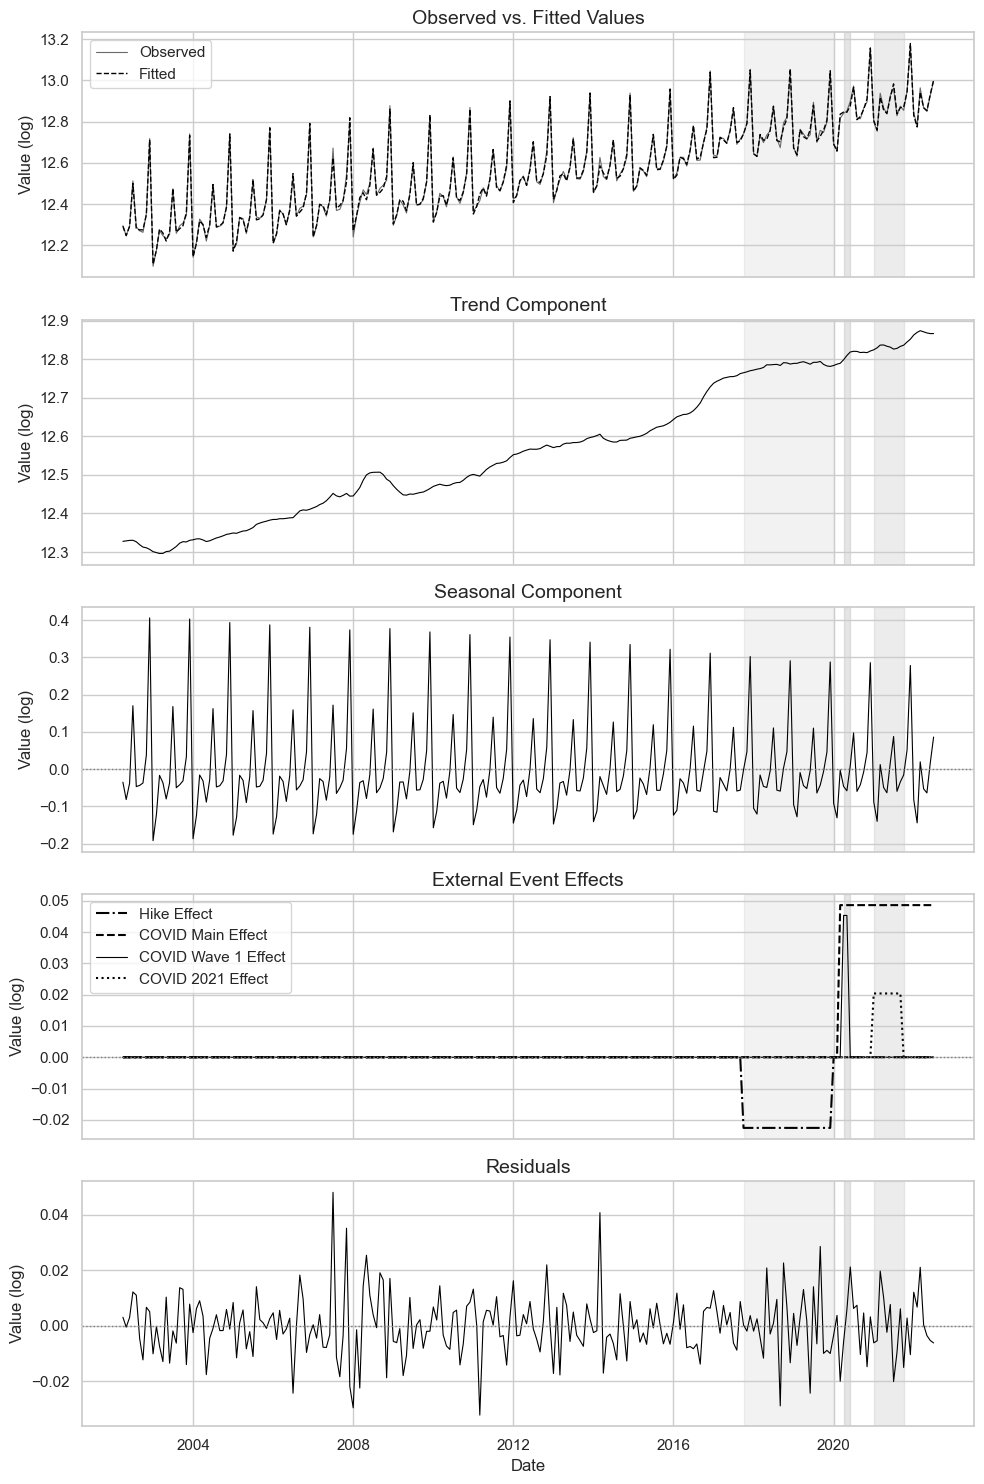
\includegraphics[width=0.5\textwidth]{../output/Decomposition.png}
  \caption{提案モデルによる時系列成分の分解}
  \label{fig:Decomposition_series}
\end{figure}

\section{考察}

\section{おわりに}

%--- 参考文献など ---
\section*{参考文献}
\noindent % インデント（字下げ）なし
[1] ○○○○(2019). 論文集用原稿の作成について、日本計算機統計学会第33回シンポジウム論文集, pp. 12-34.

\end{document}